\documentclass{article}
\usepackage{tikz}

\begin{document}

\tikzstyle{every node}=[circle, draw, fill=red, inner sep=0pt, minimum width=4pt]

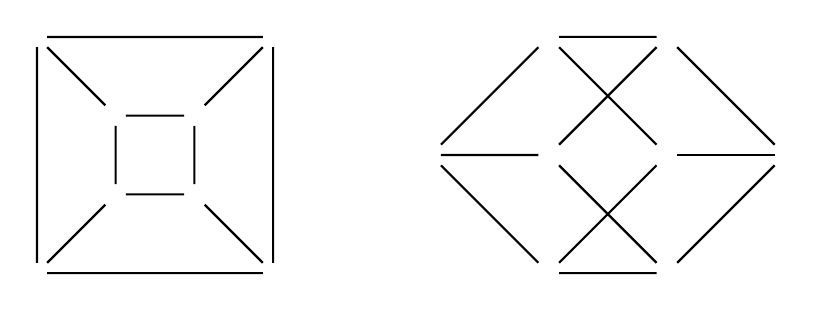
\begin{tikzpicture}[thick]
  \node (a) at (0,0) {};
  \node (b) at (0,3) {};
  \node (c) at (3,3) {};
  \node (d) at (3,0) {};
  \node (e) at (1,1) {};
  \node (f) at (1,2) {};
  \node (g) at (2,2) {};
  \node (h) at (2,1) {};

  \draw (a)--(b)--(c)--(d)--(a)--(e)--(f)--(g)--(h)--(e);
  \draw (b)--(f);
  \draw (c)--(g);
  \draw (d)--(h);

  \begin{scope}[xshift=5cm, yshift=1.5cm, scale=1.5]
  \node (a) at (0,0) {};
  \node (b) at (1,1) {};
  \node (c) at (2,0) {};
  \node (d) at (1,-1) {};
  \node (e) at (1,0) {};
  \node (f) at (2,1) {};
  \node (g) at (3,0) {};
  \node (h) at (2,-1) {};

  \draw (a)--(b)--(c)--(d)--(a)--(e)--(f)--(g)--(h)--(e);
  \draw (b)--(f);
  \draw (c)--(g);
  \draw (d)--(h);



    \end{scope}

\end{tikzpicture}




\end{document}
